\chapter{The cross cultural \\ cost of errors} 

\label{Chapter 7}

\lhead{Chapter 7. \emph{Cross cultural cost of errors}}
\vspace{3cm}
\newpage

% New Sections for Ami to read
% - Introduction that joins from last chapter: highlighted red. 

\noindent
The method, results and discussion of this Chapter appear in the submitted manuscript `The cross cultural cost of errors: the mental representation of familiar and unfamiliar numerals across cultures' \cite{garrettWheel1}. 

\color{\Red}
\section{Chapter overview}
In the previous Chapter, we assessed the mental representations of symbolic (Arabic, Chinese and Thai) and non-symbolic (dots) numerals in an English speaking cohort. We observed differences between the mental representations of symbolic numerals, and considered the effect of familiarity on the mental space. In this Chapter we will extend this investigation to a Chinese speaking cohort. The first aim of this Chapter is to examine the mental representations of the same numeric stimuli within a Chinese speaking cohort. The second aim of this study is to contrast the mental representations of the Chinese speaking and English speaking cohorts, and examine how familiarity with a numeric-set changes representations within the mental space. The background literature and methods for this Chapter are nearly identical to the previous Chapter. For this reason, we provide a relatively brief introduction to this Chapter and focus the methods of the aspects that differed from the previous Chapter, before we move onto our results and discussion. 

\section{Introduction}
Human civilisations are shaped by the communication of ideas, emotions and quantities. The ability to accurately communicate quantity has been integral to the advancement of mathematics, finance, agriculture, engineering, and warfare. The importance of accurately communicating quantity has led many cultures to develop their own symbolic numeral systems. For example, the Arabic numerals 0 -- 9 and the Chinese numerals \begin{CJK}{UTF8}{gbsn} 〇 -- 九\end{CJK}. 

Physical similarities between two numerals, for example 2 and 7, or the numerical proximity between two numerals, for example 5 and 6, may lead us to confuse the identify of one numeral with another. The cost of these confusions could be small, for example, confusing \$5 as \$6, or life-changing, for example, confusing 3 with 8 on your winning lottery ticket! These confusion patterns are intimately tied to our internal mental representations, and these representations may change across cultures. As we showed in the previous Chapter, by modelling confusion patterns, we can assess these internal mental representations and determine how and why we confuse familiar and unfamiliar numeric sets.

Our internal representation of a numeric set depends on %upon 
our experience. Whether we interpret numerals as unique symbols or numeric values, depends on our familiarity with the numeric set. For example, Chinese numerals are used regularly in Chinese speaking cultures to represent quantity, but are uncommon in predominantly English speaking cultures. These differences might change how Chinese numerals are represented in the mental space between these two cultures. By contrast, non-symbolic dots, as found on domino tiles, playing cards and dice, are a direct representation of quantity and may have similar mental representations across cultures. But what effect does expertise have on the mental representation of numerals? 

The current study investigates the effect of perceptual similarity and numerical proximity on the confusion of numerals within a Chinese speaking cohort. We analyzed confusion patterns in a digit-identification task (via confusion matrices) and assessed how perceptual and numerical properties influenced the mental representation of familiar and unfamiliar digits. We also considered the mental representation of non-symbolic quantities, such as dice patterns. Finally, we compared the results of the current study to those of a previously collected English speaking cohort, reported in Chapter 6. To foreshadow, we find evidence that symbolic numerals are confused by perceptual similarities, and quantities are confused by perceptual similarity and numerical proximity. Additionally, we find evidence that expertise changes the mental representation of Chinese numerals between the Chinese speaking and English speaking cohorts. 
\color{black}

\subsection{Expertise and the mental space}
In their investigation of symbolic similarity, \citeA{yeh2003role} presented participants with Chinese characters and asked them to spatially arranged the characters by similarity. The spatial arrangement of the Chinese characters was thought to represent similarity or proximity within the mental space. Taiwanese and Japanese students who were familiar with Chinese characters arranged items by configurable structures, treating them as whole objects and focusing upon global perceptual similarities. By contrast, English and illiterate Taiwanese students arranged items by localised feature components, for example, individual line strokes and line orientations. Although the semantic content of the letters had no effect on the literate group, familiarity and expertise altered how these Chinese characters were perceived between the two groups. 

The way we perceive an item may change with our level of expertise. With experience, some stimuli such as faces \cite{taubert2011role}, fingerprints \cite{busey2005behavioral}, cars \cite{gauthier2003perceptual} and experimentally controlled objects \cite{chua2019domain}, may be examined through a holistic visual process. Holistic processing is the obligatory attention to all parts of an object, for example, processing a ‘face’ before the composite eyes, mouth and nose. Holistic visual processing is thought to develop with experience and is both stimulus and context specific \cite{chua2019domain}. Holistic visual processing is in direct contrast to part-based visual processing, where each feature of an object is visually examined in sequence. 

In \citeauthor{yeh2003role}'s (2003) study, it is possible that experienced participants progressed from a part-based to a holistic visual processing strategy. This would explain why they focused upon holistic differences while the novice group focused upon localised line strokes. \citeauthor{yeh2003role}'s finding, and the theoretical transition from part-based to holistic processing, provides compelling evidence that the visual processing of numerals --- and their representations in the mental space --- may change with expertise. The methodology used by \citeauthor{yeh2003role} has since been applied to study the mental representation of numerals in an English speaking cohort.

\citeA{godwin2014numSim} applied the spatial arrangement method to study the mental representation of Arabic numerals in an English speaking cohort. Through multidimensional scaling (MDS), a method used to visually represent the dimensional properties of confusion patterns, \citeA{godwin2014numSim} found Arabic numerals were represented along two perceptual dimensions: i) `roundness' and `straightness', for example 3 vs 8 are more similar than 3 vs 7,  and ii) `openness', for example 2 vs 7 are more similar than 2 vs 1. Importantly, even though the tested cohort were familiar with Arabic numerals, numerical proximity had no influence on these mental representations. 

The work of \citeA{yeh2003role} and \citeA{godwin2014numSim} establish three important points. They show that numeral processing is affected by expertise, that this expertise alters how we perceive stimuli, and that numeric stimuli are not necessarily influenced by their semantic value. Our findings from the previous Chapter align with these assertions. 

\subsection{Extending Chapter 6}
In the previous Chapter, we found evidence that an English speaking cohort confused familiar Arabic digits along dimensions of perceptual similarity, and displayed no influence of numerical proximity. Furthermore, we observed that unfamiliar Thai digits were confused along dimensions of perceptual similarity, and that non-symbolic dots were confused along dimensions of perceptual similarity and numerical proximity. Given similar levels of expertise, we should expect these findings to translate to a Chinese speaking cohort.

Similar levels of expertise should result in similar mental representations for symbolic and non-symbolic digits. Arabic and dot numerals are familiar to both Chinese and English speaking cohorts. Thai numerals are unfamiliar to both cohorts. As these numeric sets share similar levels of expertise across English and Chinese speaking cohorts, we should observe similar mental representations. By contrast, Chinese numerals are only familiar to the Chinese speaking cohort. Therefore, the mental representations of this numeric set should differ between the two cohorts.

In the current study, we will extend the work of the previous Chapter and examine the mental representation of familiar and unfamiliar numerals in a Chinese speaking cohort. We will then examine the effect of expertise on the mental space by comparing the results of the current study to the results of the English speaking cohort from the previous Chapter.

\subsection{The current study}
In a Chinese speaking cohort, we combined a method for removing response bias using Luce's choice model with multidimensional scaling to assess the mental representation of digits from four different numeric-types: Arabic, Chinese, Thai and non-symbolic dots. In line with results from our previous investigation, we hypothesized symbolic numerals (Arabic, Chinese and Thai) would be confused by dimensions of perceptual similarity, and that non-symbolic dots would be confused by dimensions of perceptual similarity and numerical proximity. In accordance with the findings of \citeA{yeh2003role}, we hypothesized that experienced Chinese speakers would confuse Chinese numerals by global or holistic visual features, and inexperienced English speakers would confuse Chinese numerals by localised visual features, for example, individual line strokes. Both cohorts were equally familiar with Arabic and dot numerals, and were equally unfamiliar with Thai numerals. We therefore hypothesized no difference between the cohorts for the mental representations of Arabic, Thai and non-symbolic dot numerals.

\section{Method}
The methods and data analysis for the current study are nearly identical to the previous Chapter. As such, we only present the methods in so far as how they differed from the previous investigation.

\subsection{Participants}
Participants were 11 (4 females) student volunteers from the National Cheng Kung University, Taiwan, who completed four 90 minute experimental sessions and were reimbursed \$150 New Taiwan dollars per hour. The average age was 21.33 years (SD = 2.64 years). All participants reported as having normal or corrected to normal vision. Five participants reported their `Test of English as a Foreign Language' \cite<TOEFL;>{laborda2009building} scores, previously administered as part of their undergraduate degrees. The average TOEFL score was 77.8 (SD = 5.26) indicating moderate-to-good English proficiency. 

\subsection{Stimuli and apparatus}
Stimuli were presented on an 18inch CRT (60Hz) monitor with a 4:3 aspect ratio at a display resolution set to 1280 x 768. The visual angle of the stimulus was matched between testing facilities (Taiwan and Australia).


\section{Results}
\subsection{Accuracy}
Signal contrast and identification accuracy was successfully manipulated at the start of each session by our modified staircase procedure. Signal contrast levels were approximately equal for Chinese (RGB $\mu$ = 137.4, $\sigma$ = 1.49)\footnote{Note, the RGB values are the same for red, green and blue values and are reported as a single number for simplicity. Hence, 137.4 actually codifies an RGB value (137.4, 137.4, 137.4).}, Arabic (RGB $\mu$ = 137.6, $\sigma$ = 1.15) and non-symbolic dot numerals (RGB $\mu$ = 137.8, $\sigma$ = 3.89), and highest (easiest) for Thai numerals (RGB $\mu$ = 140.3, $\sigma$ = 1.75). This difference may reflect the unfamiliar nature of the Thai numeric set. A full statistical analysis of the calibration block and staircase procedure is included in supplementary material S5\ref{Appendix:Staircase}.

Experimental accuracy was successfully manipulated by displaying stimuli at five levels of signal-contrast. Across numeric types, mean accuracy increased linearly with the visibility of the contrast levels. Accuracy was lowest at level 1 (easiest; $\mu$ = .48, $\sigma$ = .17) and highest at level 5 (hardest; $\mu$ = .79, $\sigma$ = .11). Across experimental trials, mean accuracy was highest for non-symbolic dots ($\mu$ = .72, $\sigma$ = .14), then Chinese numerals ($\mu$ = .66, $\sigma$ = .12), Arabic numerals ($\mu$ = .62, $\sigma$ = .14), and finally, Thai numerals ($\mu$ = .59, $\sigma$ = .11). A full statistical analysis of experimental accuracy is included in supplementary material S5\ref{Appendix:Accuracy}.

\subsection{Response bias}
A Pearson rank-order correlation displayed a positive relationship between the frequency of stimulus responses (strength in Luce's choice model) and stimulus accuracy. This correlation held for Arabic numerals ($r$ = .57, $p < $ .001), Chinese numerals ($r$ = .59, $p < $ .001), Thai numerals ($r$ = .58, $p < $ .001) and non-symbolic dots ($r$ = .61, $p < $ .001). Results indicate that stimulus accuracy might be influenced by the frequency of responding and response bias (a full analysis of response bias is included in supplementary material S5\ref{Appendix:Bias}). To remove the confound of response bias from the confusion data, we applied Luce's similarity choice model. In the following section, we will consider the effect of response bias on the mental representation of numerals. We will use MDS to visualise relative item proximities in the mental space for biased (uncorrected) and bias-free MDS solutions.

\subsection{Biased to bias-free MDS}
Figure \ref{fig:Bias2Biasfree} shows MDS results from a representative data set (participant S3) where response-bias was unaccounted for (biased plots) and corresponding MDS results where response-bias was removed from the data using Luce's choice model (bias-free plots). Changes between item-proximities within each numeric-type (black arrow) illustrates how the removal of response-bias alters the MDS solution. Item proximities did not change where response bias had little impact, for example, the proximity between dot numerals 8 and 9 did not shift between uncorrected and corrected MDS solutions. By contrast, item proximities shifted dramatically when response bias altered the mental space, for example, Arabic numerals 5 and 8. All future references to MDS within the results section will pertain to the bias-free MDS solutions.

\begin{figure}[tbh]
\centering 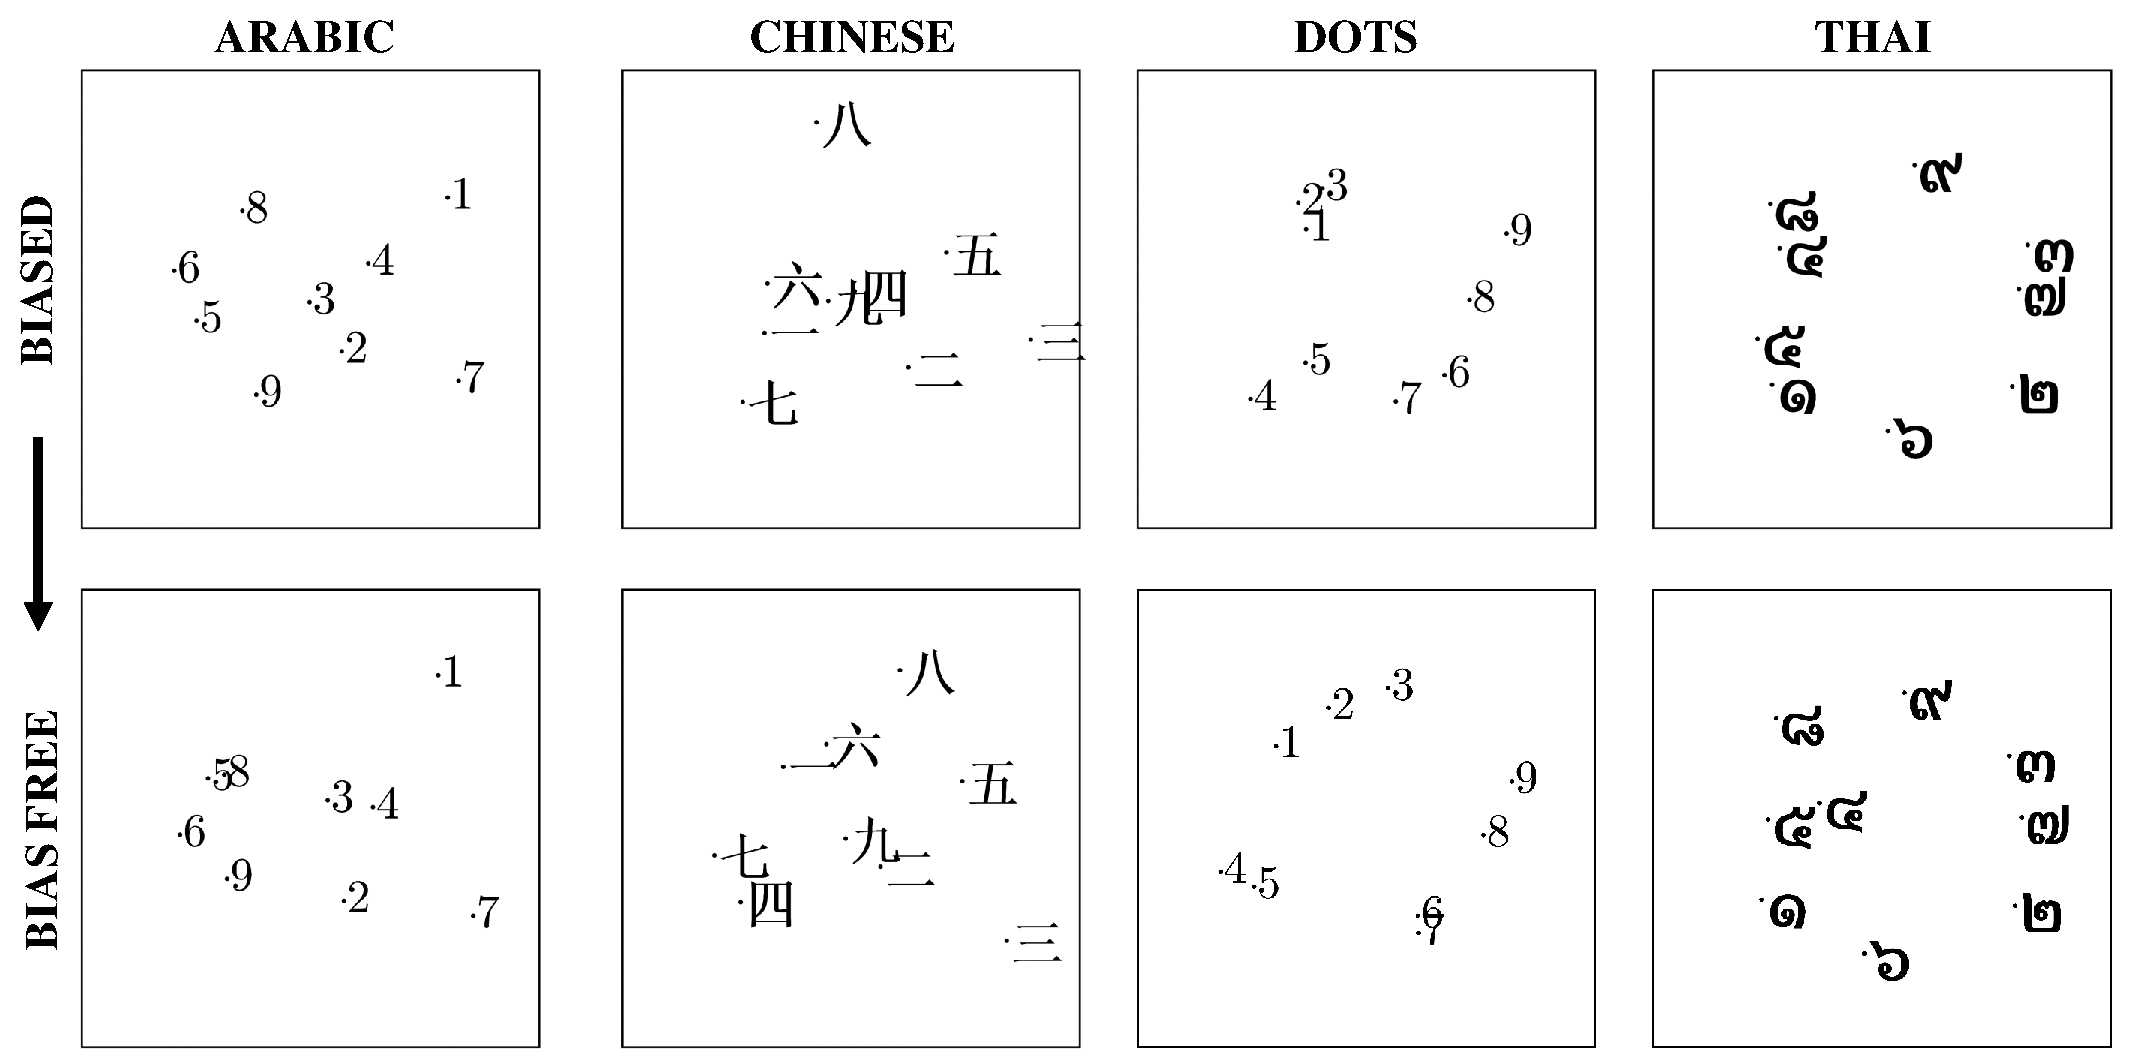
\includegraphics[width = \linewidth]{Figures/CrossWheel/Bias2BiasFree.pdf}
\caption{Biased (uncorrected) and bias free (Luce's choice model corrected) MDS solutions for participant S3, displayed separately for each numeric-type. Changes in item-proximity between biased and bias-free MDS plots display the effect of response-bias on the MDS solution. \\\textbf{Note.} Dots are presented as Arabic numerals to avoid misinterpretation due to spatial overlap.}
\label{fig:Bias2Biasfree}
\end{figure}

\subsection{MDS}
Scree analysis identified two-dimensions as the best MDS representation for most participants in each numeric-type (see supplementary material S5, Figure \ref{fig:Apx_ScreeEngDot_Cross} and Figure \ref{fig:Apx_ScreeChnThi_Cross}). Scree analysis identified three-dimensions as the appropriate MDS representation for one participant in the non-symbolic dots numeric-type, two participants in the Chinese numeric-type, and three participants for the Thai numeric-type. Individual bias-free MDS plots are displayed in supplementary material S5, Figure \ref{fig:Apx_MDSenglish_Cross} -- Figure \ref{fig:Apx_MDSthai_Cross}, and uncorrected MDS plots are displayed in supplementary material S5, Figure \ref{fig:Apx_MDSenglishBiased_Cross} -- Figure \ref{fig:Apx_MDSthaiBiased_Cross}. To describe trends observed across participants, we conducted an Individual Differences Scaling (indscal) MDS analysis. For efficiency of exposition, and as only a select few participants displayed three-dimensional MDS solutions, the following results will focus on the two-dimensional group indscal results.

\subsection{Indscal results}
Figure \ref{fig:Indscal_Cross} (left) displays the two dimensional group indscal MDS solutions for each numeric type. Interpretation of MDS plots is at times arbitrary and relies on visual inspection of the plots. Similarly, interpretation of the MDS solution's axes are also arbitrary with reference to the x- or y-axes \cite<see e.g.,>{nosofsky1986attention, nosofsky2018toward}. Likewise, the notion of similarity is very broad and has been the centre of many disputes in the literature \cite<e.g.,>{tversky1977features, medin1993respects}. To simplify this process, the apparent MDS dimensions have been labelled with directional arrows for each plot. Determining which items cluster together, and the strength of their association in the MDS space is a difficult task. We have formalized this process with an analysis of K-mean clustering. 

\begin{figure}[tbh]
\centering 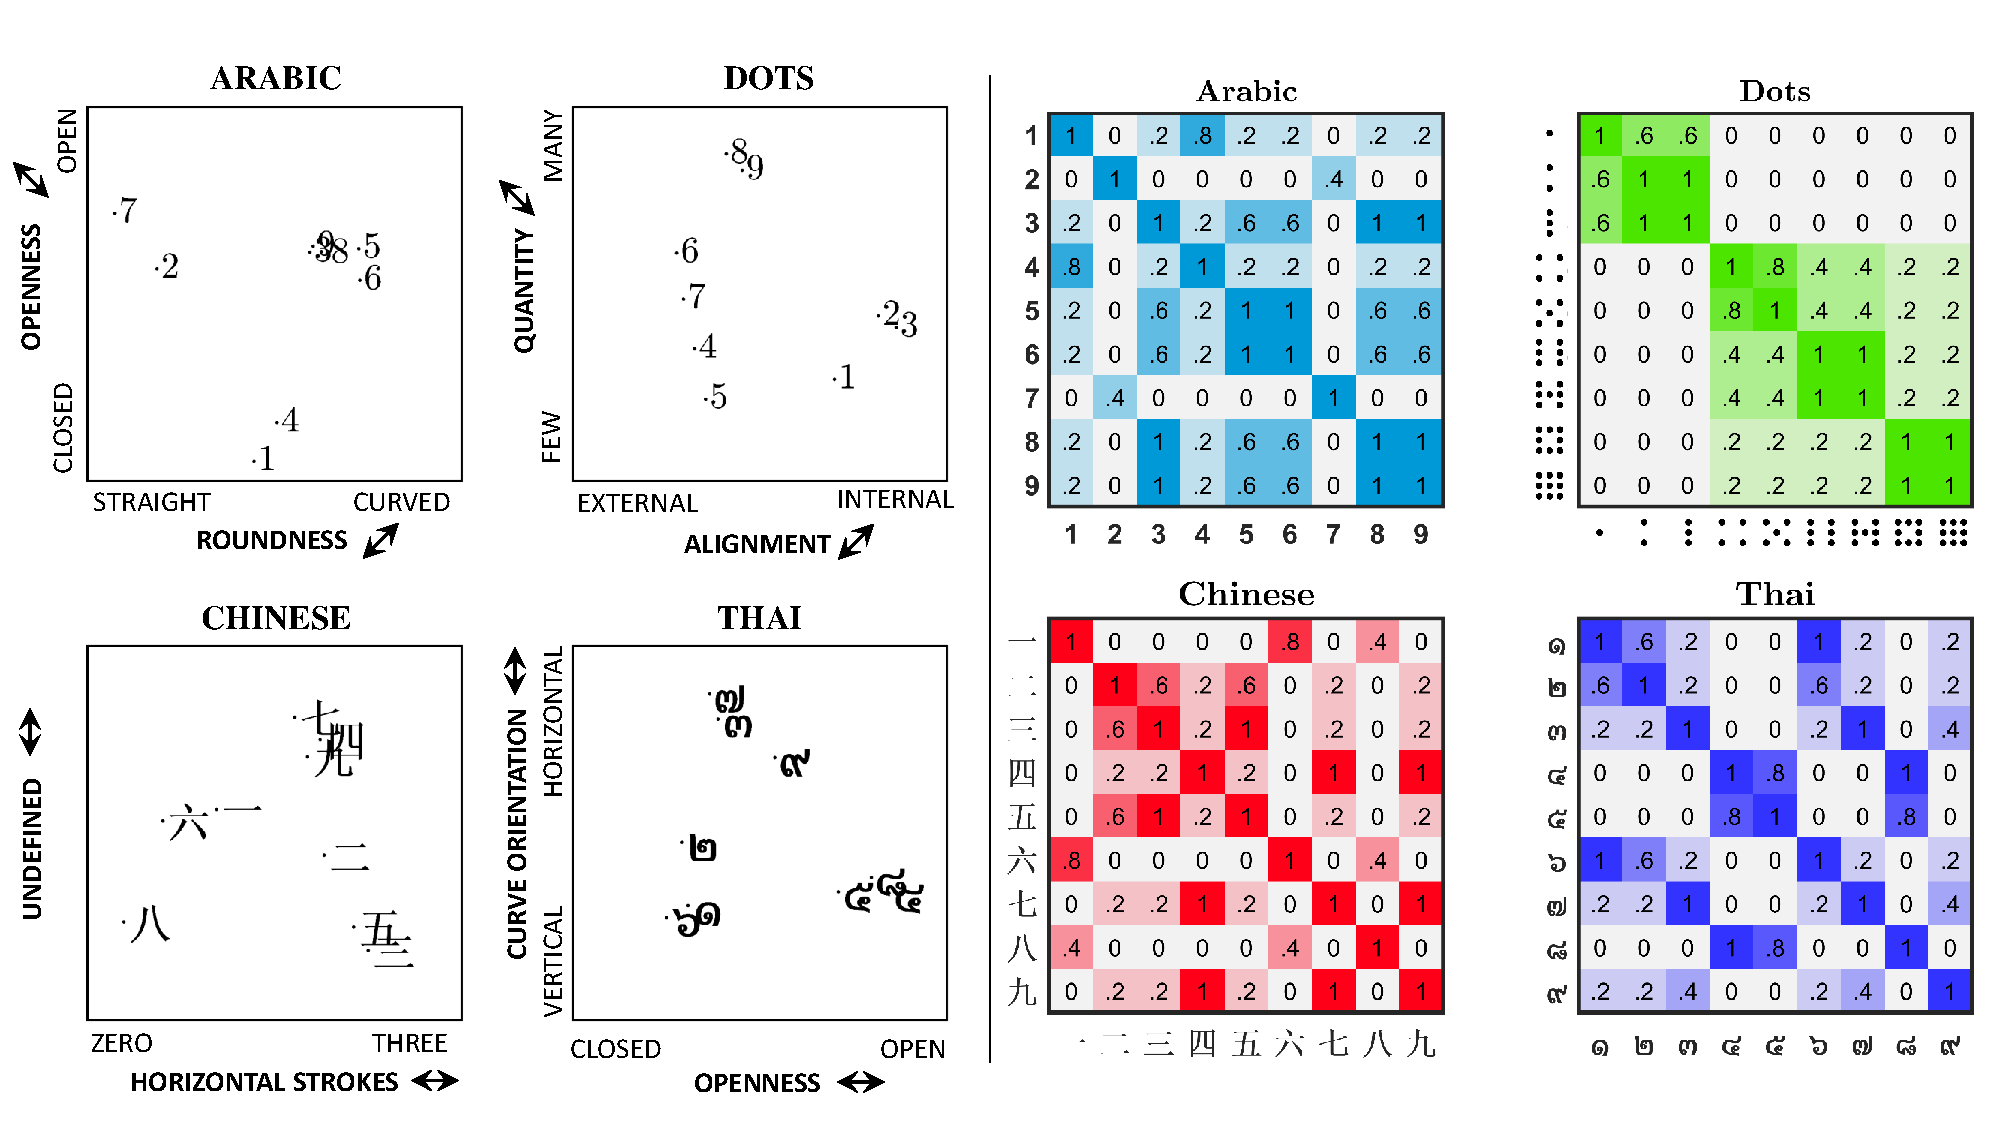
\includegraphics[width = \linewidth]{Figures/CrossWheel/Indscal2D.pdf}
\caption{Left: Individual differences scaling (indscal) solution for all participants best represented by a two-dimensional MDS space, displayed separately for each language-type. Dimensional labels and directionality (arrows) are displayed on the y-axis and x-axis. Right: Proportional cluster-frequency heatmap for MDS indscal results, across 2--6 K-mean clusters. Larger proportions (darker colors) indicate items which cluster most frequently.}
\label{fig:Indscal_Cross}
\end{figure}

Figure \ref{fig:Indscal_Cross} (right) displays an MDS cluster frequency heatmap. For each MDS solution, a K-mean cluster analysis was performed using 2--6 clusters. The proportion at which any two items clustered was calculated for each iteration of K. Where two items clustered on every iteration of K, (\eg Arabic numerals 3 and 8), the proportional frequency was 1. Conversely, where two items never clustered, (\eg Arabic numerals 1 and 2), the proportional frequency was 0. The combination of these methods provides i) a description of the MDS dimensions, and ii) a measure of item similarity strength. This technique provides quantifiable conclusions about item clusters, rather than subjective interpretations. 

Arabic numerals appeared to be represented along two perceptual dimensions of similarity: openness and roundness \cite<similar results were observed by>{godwin2014numSim}. Openness describes the concave absence within a numeral, and roundness describes the curvature of a numeral. Cluster frequency analysis shows strong item-clusters between [3, 8, 9], [1, 4] and [5, 6]. These items all share similar degrees of roundness. Although items [2, 7] grouped within the MDS space, these items did not show a high cluster strength relative to the other groups. The location and proximity of Arabic numerals within the MDS space display no effect of numerical proximity. 

Non-symbolic dots appeared to be represented along the perceptual dimension of alignment, and the numeric dimension of quantity. Alignment describes the positions of dots within the 3 x 3 stimulus array: items 1--3 are centrally aligned, 4--7 are externally aligned, and items 8--9 are both internally and externally aligned. Quantity describes the number of items within the stimulus array. Item clusters present as staggered item-sets, with strong clusters between items [2, 3], [4, 5], [6, 7] and [8, 9]. Item 1 clustered most frequently with items [2, 3], but did not display the same level of cluster strength as the other groups. 



Chinese numerals appeared to be represented along one perceptual dimension that counted the number of horizontal strokes, and a second undefined perceptual dimension. This undefined dimension appears perceptual in origin and displays no apparent influence of numerical proximity. It is possible this dimension is a mixture of different mental representations and therefore cannot be classified at the group level. Individual MDS analyses suggest this could be the case (see supplementary material S5, Figure \ref{fig:Apx_MDSchinese_Cross}). Alternatively, this dimension might reflect a holistic visual process that integrates a range of different perceptual features and cannot be captured by the current scaling method. Item-clusters were strong for numerals \begin{CJK}{UTF8}{gbsn}[四, 七, 九]\end{CJK}, and for numerals that shared similar horizontal stroke counts, for example, \begin{CJK}{UTF8}{gbsn}[一, 六] and [三, 五]\end{CJK}.

Thai numerals appeared to be represented along perceptual dimensions of openness and curve orientation. Curve orientation describes whether Thai numerals had a vertically or horizontally aligned curved feature. Openness describes the concave absence within a numeral. Strong clusters were present between items numbers [1, 6], [3, 7] and [4, 5, 8]. These items all shared features of both openness, and curve orientation. Item number 2 was moderately clustered with items [1, 6], and item number 9 remained independent. 

\subsection{Ideal observer}
The current MDS analysis has made several interpretations based upon dimensions of perceptual similarity. The interpretation of MDS dimensions is a subjective process that may be made stronger by comparing results with an objective benchmark. To this end, we compared the current results to that of the previously conducted ideal observer analysis (Chapter 6). A summary of these results are reported here. A full breakdown is reported in supplementary material S5\ref{Appendix:IOA}. 

MDS and cluster frequency results from the ideal observer displayed very few similarities to our empirical findings. The ideal observer failed to capture the intangible dimension of `openness' and differed greatly from the Arabic and Thai numeral MDS results. Similarly, Chinese numeral MDS results differed greatly between the ideal observer and empirical findings. Finally, ideal observer results were very different for non-symbolic dots, however, as empirical results displayed a combined effect of perceptual similarity and numerical proximity, this finding is to be expected. Together, these results suggest the perceptual dimensions observed in the empirical data go beyond that of simple low level perceptual similarities and reflect higher level dimensions of perceptual similarity, (e.g., openness).

\section{Interim discussion}
Accuracy was successfully manipulated through our staircase procedure. The resulting confusion patterns were subject to Luce's choice model and confusion scores were corrected for the confound of response bias. In line with our hypotheses, MDS indscal and cluster frequency analyses showed that symbolic numerals (Arabic, Chinese, and Thai) appeared to be confused along dimensions of perceptual similarity in the mental space. As predicted, non-symbolic dots appeared to be confused along dimensions of numerical proximity and perceptual similarity in the mental space.

In keeping with our expectations, symbolic numerals appeared to be represented by perceptual dimensions of similarity in the mental space. Familiarity with the Arabic and Chinese numeral sets did not promote an effect of numerical proximity, (i.e., numerical distance). Thai numerals were unfamiliar to the current cohort and as expected, were only confused by dimensions of perceptual similarity. 

In keeping with our previous investigation \cite{garrettWheelTask}, non-symbolic dots appeared to be represented by dimensions of perceptual similarity and numerical proximity within the mental space. There was a clear numerical distance effect --- numerically closer items were confused more often than items further apart. However, this effect was confounded by perceptual similarity and produced staggered item clusters. For example, items [2, 3] and [4, 5] always clustered together, but never items [3, 4] or [5, 6]. Staggered item-clusters only varied by the presence or absence of a single central dot. This means an alternative account of the data could be that numerical proximity confounded the effect of perceptual similarity, producing staggered item-clusters. The co-variation between quantity and perceptual features makes it impossible to disentangle the effects of these dimensions in the mental space using the current results. For now, we may only conclude that dot numerals were confused along dimensions of quantity and alignment, supporting a combined effect of numerical proximity and perceptual similarity on the mental space.

Although the results of the current study aligned with our hypotheses, there are compelling reasons to believe the mental representation of numerals, specifically how numerals are perceived, might change with expertise. For example, the current study employed a Chinese speaking cohort who were familiar with Chinese numerals. This familiarity might alter the perception of Chinese numerals, relative to an inexperienced or naive cohort \cite<e.g.,>{yeh2003role}. To this end, we now compare the results of the current study to the results of the English speaking cohort as presented in the previous Chapter. 


\section{Cohort comparison results}
\subsection{Accuracy}
Mean accuracy was comparable between cohorts for each numeric-type, and error rates were sufficient for MDS analysis. On average, the Chinese speaking cohort was more accurate ($\mu$ = .65, $\sigma$ = .12) than the English-speaking cohort ($\mu$ = .58, $\sigma$ = .14), a trend that held within each numeric-type. On average, the English speaking cohort was most accurate for non-symbolic dots ($\mu$ = .65, $\sigma$ = .12), Thai numerals ($\mu$ = .64, $\sigma$ = .1), Chinese numerals ($\mu$ = .61, $\sigma$ = .15), and finally Arabic numerals ($\mu$ = .55, $\sigma$ = .15). A direct comparison of accuracy between cohorts is difficult due to the differences between testing facilities. Each testing facility employed different monitors (CRT vs LCD) and ambient lighting. This produced similar levels of accuracy between the two cohorts, at different signal contrast levels.


Figure \ref{fig:ComparedAccuracy} displays the matched signal-contrast accuracy for the Chinese speaking cohort (left) and the English speaking cohort (right). Participants viewed stimuli at five levels of signal contrast and the average accuracy for each of these signal-levels is plotted Figure \ref{fig:ComparedAccuracy}. For example, if for Arabic numerals, participant S1 viewed stimuli at RGB values 134--137, and participant S2 viewed stimuli at RGB values 137--141, their accuracy at the shared contrast value of 137 would be averaged and plotted in the figure. By matching accuracy across contrast-levels, we may compare accuracy trends for each numeric-type within each cohort. This method also allows us to compare accuracy trends between cohorts by comparing the relative ordering of the numeric-types. Differences between the actual contrast levels reflect perceptual differences incurred at each testing facility.

\begin{figure}[tbh]
\centering \includegraphics[width=\linewidth]{Figures/CrossWheel/Comparison_AccuracySubplot.jpg}
\caption{Mean accuracy matched by contrast-level for the Chinese speaking cohort (left) and English speaking cohort (right) across numeric types. Note, only RGB values with multiple data points are displayed. Error bars represent one standard-error of the mean.}
\label{fig:ComparedAccuracy}
\end{figure}

When accuracy was matched by signal contrast level, unfamiliar Thai numerals displayed the lowest accuracy trends across both cohorts. Within the Chinese speaking cohort, non-symbolic dots displayed the highest level of accuracy at lower contrast levels, and crossed over with Arabic and Chinese numeral accuracy trends at higher contrast levels. Arabic and Chinese numerals displayed comparable accuracy across the range of contrast levels. Within the English speaking cohort, non-symbolic dots and Arabic numerals displayed similar trends in accuracy across the range of contrast levels, and were slightly more accurate than Chinese numerals. These results display a trend whereby familiar numerals within each cohort were responded to with greater accuracy than unfamiliar numerals, given the same level of signal contrast. 

\subsection{Confusion scores}
Confusion scores, the rate at which one numeral is erroneously confused with another, index proximity between items in the mental space. If confusions are strongly correlated between cohorts, similar representations may exist between the mental spaces of each cohort. We calculated the Pearson's correlation ($r$) between cohort confusion scores for each numeric type, after setting the main diagonal (accurate identifications) to zero. This was done for the uncorrected (biased) confusion scores, and the bias-free confusion scores. 

Uncorrected confusion scores, (i.e., confusions scores before the application of Luce's choice model) were highly correlated for Arabic ($r$ = .9, $p <$ .001), non-symbolic dot ($r$ = .9, $p <$ .001), Thai ($r$ = .89, $p <$ .001) and Chinese numerals ($r$ = .87, $p <$ .001). These correlations increased with the removal of response-bias for Arabic ($r$ = .94, $p <$ .001), non-symbolic dot ($r$ = .97, $p <$ .001), Chinese ($r$ = .92, $p <$ .001), and Thai numerals ($r$ = .95, $p <$ .001). The correlation of bias free confusion scores suggests that, between cohorts, the mental space is most similar for non-symbolic dots, than Thai numerals, Arabic numerals and finally, Chinese numerals. Further examination of the similarities and differences between the mental representations of each cohort requires MDS comparisons.

\subsection{MDS comparison}
Figure \ref{fig:IndscalCompared_Procrustes} displays the group MDS indscal solutions for the Chinese-speaking cohort (left column) and English-speaking cohort (middle column). The apparent dimensions along which numerals were represented in the mental space are displayed along the x- and y-axes. Similar dimensions were observed between cohorts for Arabic numerals (openness vs roundness), non-symbolic dots (quantity vs alignment) and Thai numerals (curve orientation vs openness). Chinese numerals were represented along different dimensions in the Chinese-speaking cohort (an undefined perceptual dimension vs the number of horizontal strokes) and English-speaking cohort (the number of line terminations vs the stroke alignment; see Figure \ref{fig:IndscalCompared_Procrustes}). To empirically assess the degree of similarity between these MDS representations, we performed a procrustes analysis on the group indscal results.

\newpage
\begin{figure}[!htb]
\centering 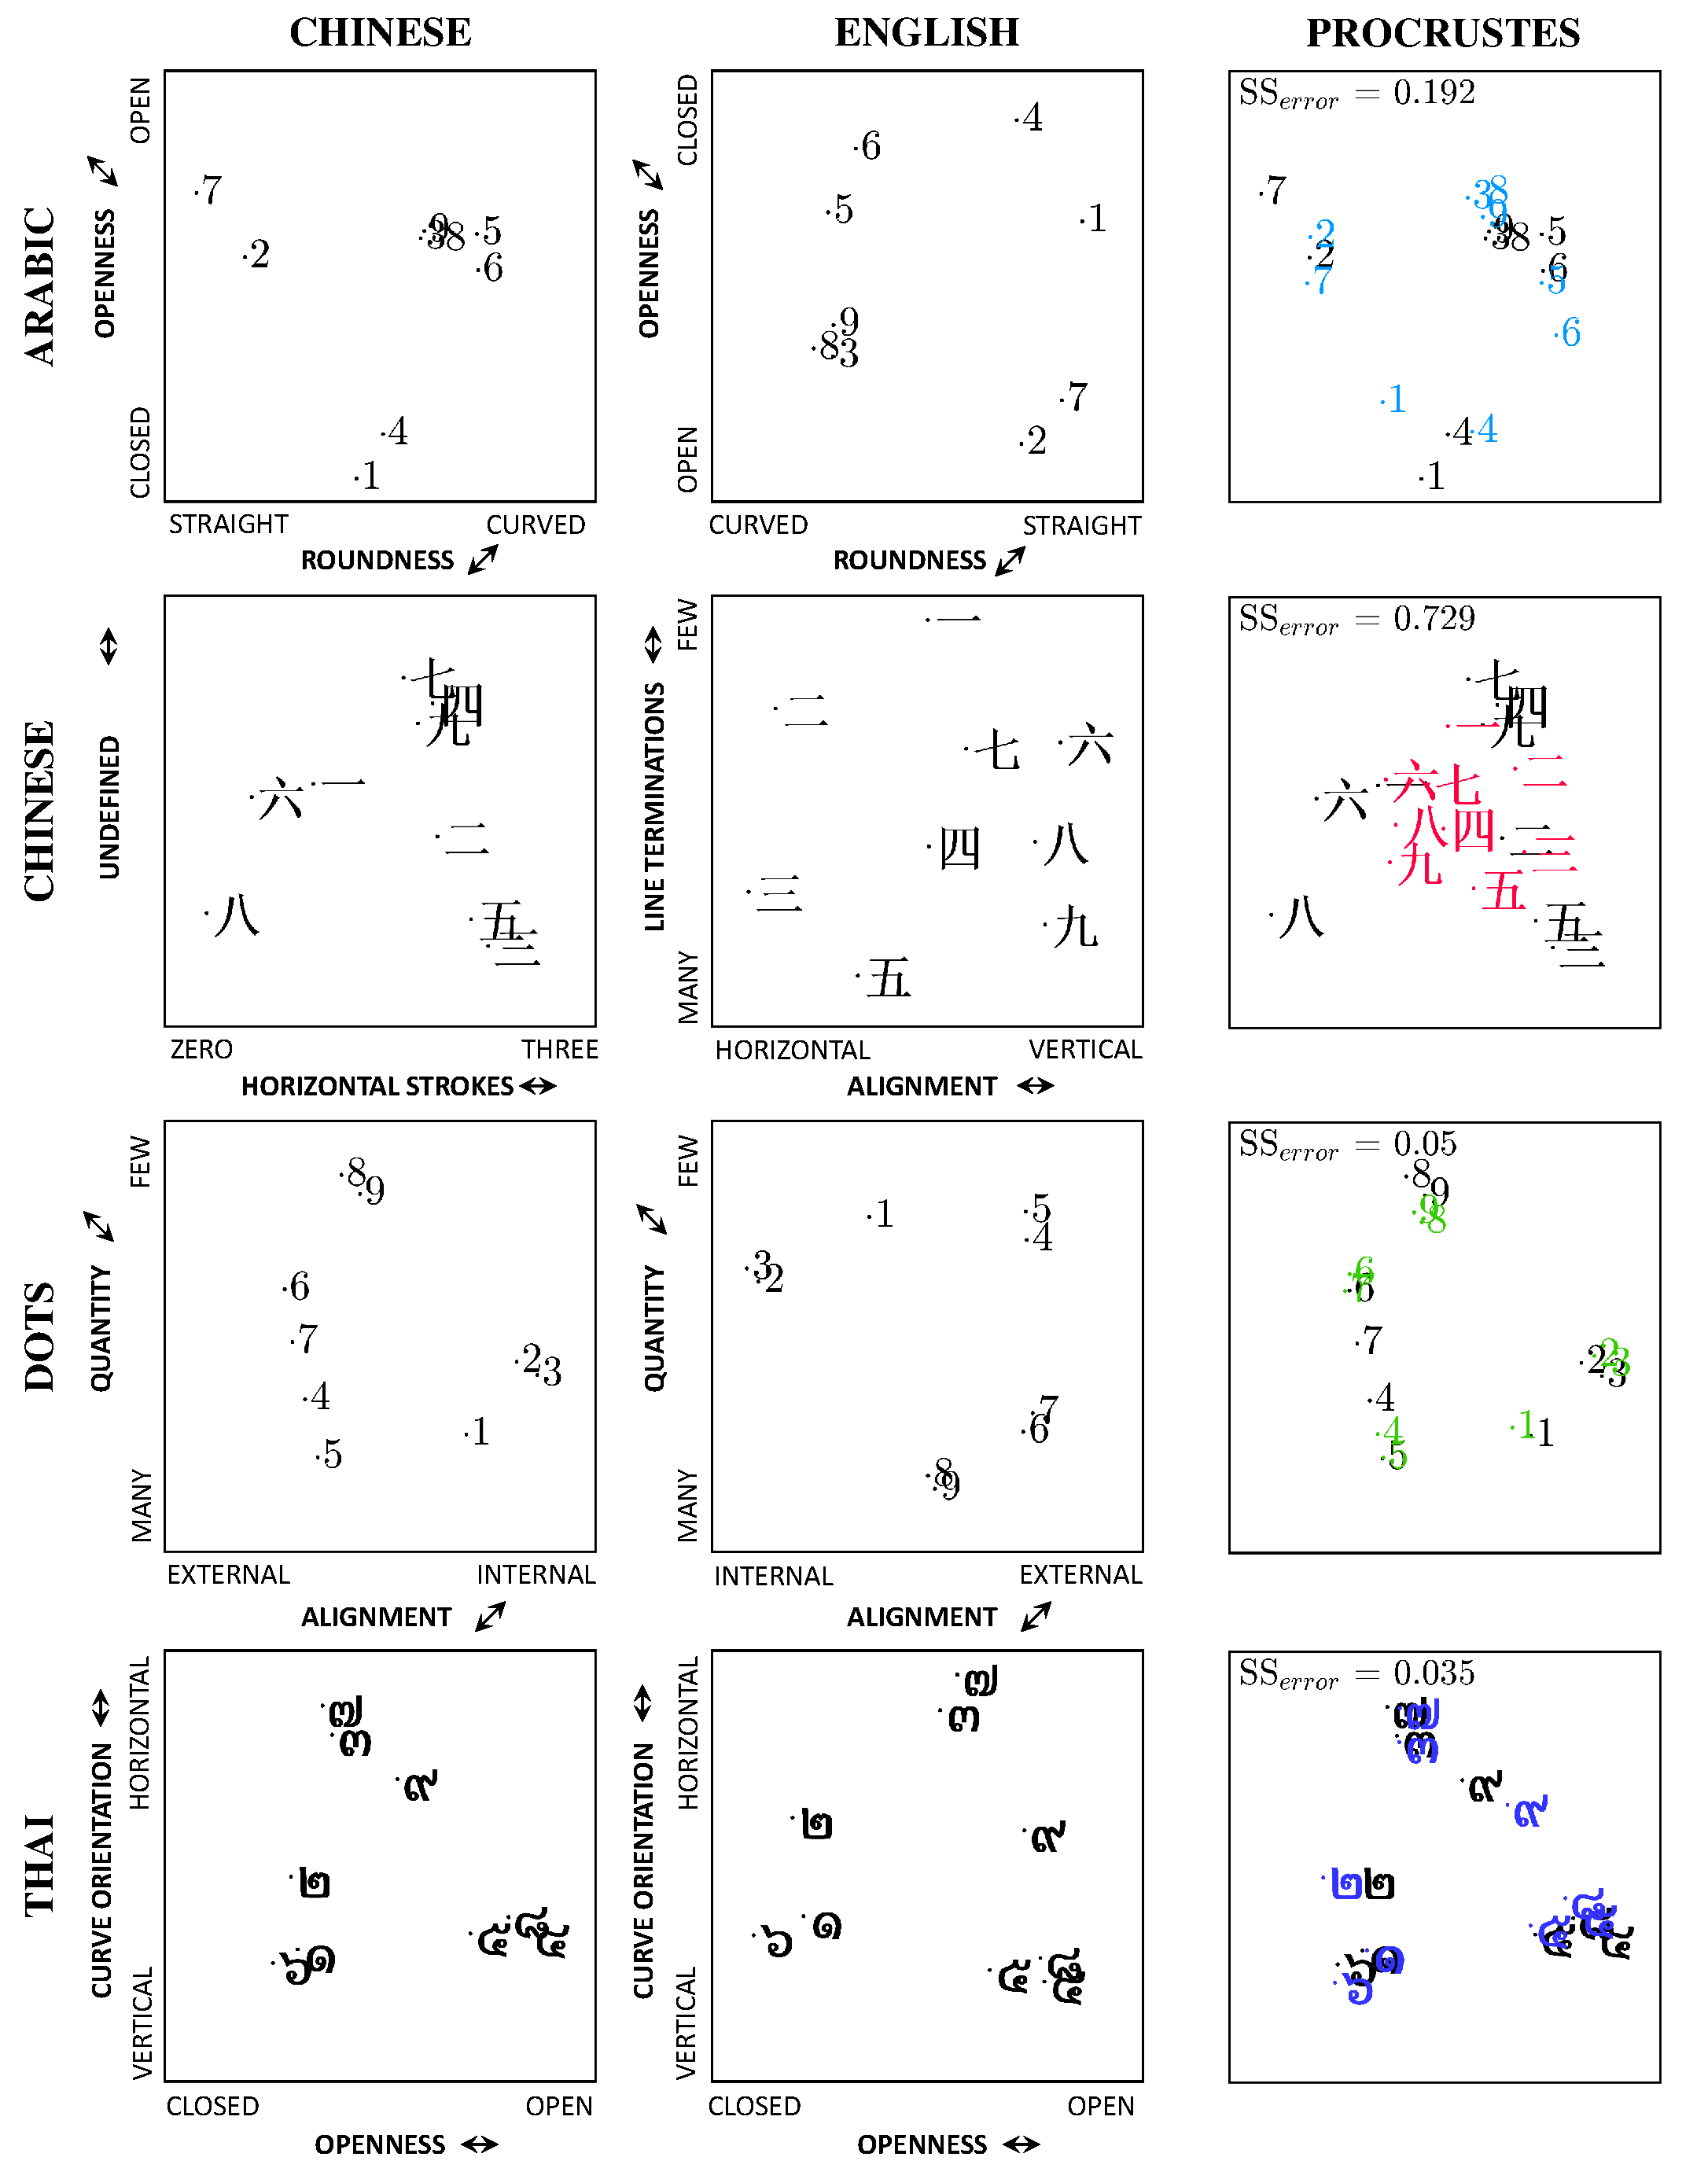
\includegraphics[width=\linewidth]{Figures/CrossWheel/IndscalCompared.pdf}
\caption{Indscal MDS solutions for the Chinese speaking cohort (left), English speaking cohort (middle) and a procrustes analysis fitting the English cohort to the Chinese cohort's MDS solutions (right). Colored items represent the English cohort's transformed MDS indscal solution fit to the Chinese MDS indscal solution. Standardised sum of squared errors (goodness of fit) is reported in the top left of each panel; a lower SS$_{error}$ indicates a better fit between cohorts.}
\label{fig:IndscalCompared_Procrustes}
\end{figure}

The procrustes analysis fits one MDS representation to another through a combination of translation (moving one over the other), rotation and scaling. A measure of fit is provided by the standardized sum of squares error. This affords a direct comparison of `goodness of fit' between numeric-types, with an SS$_{error}$ closer to zero indicating a better procrustes fit. The right column of Figure \ref{fig:IndscalCompared_Procrustes} displays the procrustes results, fitting the English-speaking cohort's MDS results (colored numerals) to the Chinese-speaking cohort's MDS results (black numerals). In line with the correlational analyses, MDS representations were most similar for non-symbolic dots (SS$_{error}$ = .05), then Thai numerals (SS$_{error}$ = .035) and Arabic numerals (SS$_{error}$ = .192). MDS results were most dissimilar for Chinese numerals (SS$_{error}$ = .729).

\section{General discussion}
When asked to identify Arabic, Chinese, Thai and dot numerals, both Chinese-speaking and English-speaking cohorts where able to complete the tasks with similar levels of accuracy. In both cohorts, familiar numeric sets were more accurately responded to than unfamiliar numeric sets, after controlling for signal-contrast. Correlational and procrustes analyses showed MDS representations were similar between cohorts for Arabic numerals, non-symbolic dots and Thai numerals. MDS representations differed between cohorts for Chinese numerals --- the only numeral set where cohorts also differed in their levels of expertise. For both cohorts, Chinese numerals appeared to be represented along dimensions of perceptual similarity, however, the perceptual features confused by each cohort differed greatly. Chinese speakers appeared to confused Chinese numerals by the number of horizontal strokes and by an undefined dimension of perceptual similarity. English  speakers appeared to confused Chinese numerals along the dimensions of character alignment and the number of line terminations. Both cohorts appeared to confuse Chinese numerals by low-level dimensions of perceptual similarity, and Chinese speakers did not show evidence of global or holistic processing relative to the English speaking cohort. 

\subsection{Expertise and the mental space}
The mental representations of Chinese numerals varied greatly between the Chinese and English speaking cohorts. Against predictions, the mental representations of Chinese speakers did not show signs of global or holistic processing. In line with predictions, the mental representations of English speakers displayed evidence of localised visual processing. Both cohorts appeared to represent Chinese numerals along dimensions of perceptual similarity, however, only the English speaking cohort were influenced by the logographic nature of the numeric set.

Chinese characters are logographic such that each character holds a unique semantic meaning. Chinese numerals are a special among these logographs, with many numerals physically symbolizing their value. For example, the Chinese characters \begin{CJK}{UTF8}{gbsn} 一, 二, 三, 四 \end{CJK} are the numerals 1--4 as indicated by the sum of their outer lines. By happenstance, Chinese numerals less-than five and greater-than five are made from predominantly horizontal and vertical line strokes, respectively. Together, these perceptual and logographic elements clearly demarcate small and large values within the range of 1--9. These influences are clearly visible within the English speaking cohort, however, are absent from the Chinese speaking cohort. 

Chinese speakers did not represent Chinese numerals by stroke alignment or the by logographic elements of the numerals. It appears that, with expertise, Chinese speakers knew to focus upon specific numeric identifiers that were not apparent to the English speaking cohort. For example, Chinese speakers appeared to focus upon the number of horizontal stroke elements. The undefined perceptual dimension within the Chinese speaking cohort might reflect a mixture of these expert visual processes. Unfortunately, this cannot be discerned from the group MDS analysis and is equally unclear at the individual level. Future investigations using our methodology might consider asking participants to describe their visual processing strategy. This may help in classifying individuals with similar MDS representations.

The results of the current study clearly show that expertise with a numeric set may change the way we perceive and represent items within the mental space. Our work adds to the established literature that examines how cognitive processes evolve with training and expertise \cite{yeh2003role, gauthier2003perceptual, chua2019domain}. Our work also shows how our mental representations can be stable across cultures given similar levels of expertise. 

\subsection{Similarities in the mental space}
The mental representations of non-symbolic dots, Thai and Arabic numerals were very similar across cohorts. Arabic and dot numerals were very familiar to both cohorts, and Thai numerals were unfamiliar to both cohorts. These similarities show that, with similar levels of expertise, stable mental representations are formed across our two cultures. 

Non-symbolic dots were most similarly represented across cohorts. This was not unexpected. Dots are a physical representation of quantity and activate the innate ANS. This numeric set validates our experimental methods and analysis techniques, producing nearly identical mental representations across both cohorts.

The mental representations for Thai numerals were the next most similar. Being unfamiliar to both cohorts, these results reflect the similar visual processes employed by both cohorts. In a future study, it would be interesting to assess the mental representation of these numeric stimuli within a Thai speaking cohort. For now, whether these stimuli are processed differently after acquiring expertise remains an unanswered question.

Arabic numerals were similarly represent across cohorts, however, to a lesser extent than Thai and non-symbolic dots. Similar mental representations were expected between cohorts, as both share similar level of expertise. However, Arabic numerals form part of a secondary language for the Chinese speaking cohort, and a primary language for the English speaking cohort. Therefore, it is possible that a small difference in expertise exists between the cohorts. This difference might explain why Arabic numerals are most different in their representations from among the non-symbolic dot, Thai and Arabic numeric types. It is fortunate and commendable that our methods and analysis techniques were able to capture this nuanced difference. 


\subsection{Future research}
The current research has shown that expertise changes the way Chinese numerals are represented within the mental space. However, the results of this study differed from our expectations \cite{yeh2003role} and may reflect a difference in methodology. We propose a future study using the spatial arrangement method \cite<as used by>{yeh2003role} in an English speaking and a Chinese speaking cohort. Using the numeric sets of the current study, participants could be asked to arrange items by perceptual similarity, and separately, by numerical proximity. Such an investigation could disentangle perceptual and semantic effects in the mental space, and determine whether the differences between the current study and \citeauthor{yeh2003role}'s investigation are due to task design. 


\subsection{Implications}
The clear communication of numeric value is important in many tasks, including finance, teaching, timekeeping and transportation. Much time can be spent crafting or selecting numeric fonts that enhance this communication. For example, it is important to have clear numeric fonts for vehicular speed signs, especially when road conditions are not ideal. The current research and methodology can be easily extended to the assessment of fonts, either within a culture, (\eg Taiwanese drivers in Taiwan), or across cultures, (\eg Australian drivers visiting Taiwan), with the aim of enhancing public safety and written communication. 

The current methodology has proven effective at examining latent cognitive dimensions (numeric proximity) between two cultures. The methods of this study could be equally applied to examine other latent dimensions, for example alphabetic proximity \cite<as shown by>{townsend1971alphabetic}, and how these latent dimensions change with expertise or due to differences between cultures. 

\section{Conclusion}
The ability to accurately communicate quantity through symbolic numerals plays an important role in all human cultures. Often, as we navigate our busy and dynamic environments, we confused the identify of one numeral for another. Such confusions provide insight into how these numeric symbols are represented within our mental space. Although past research has examined the mental dimensions of numeric item-sets, these assessments were confounded by participant response bias. We have presented bias free mental representations of familiar and unfamiliar numeric-sets in both Chinese-speaking and English-speaking cohorts. We have shown how expertise with a language-set may change the representation of numerals within the mental-space. We have also shown clear similarities in the mental representations of two different cohorts, for familiar (Arabic and dot) and unfamiliar (Thai) numerals. While expertise with a numeric set may change our mental landscape, we show that when items are novel (unfamiliar) or universally understood across cultures (symbolic dots), our mental representations are essentially the same. 

% AMI DONE 1/11/2019
